\documentclass{../../oss-apphys-exam}
%\usepackage{bm}
\newcounter{lastmc}

\begin{document}
\genheader

\gentitle{1}{KINEMATICS}

%\genmultidirections
%\gengravity

\raggedcolumns

\begin{multicols*}{2}
  \begin{questions}
    \question A golf ball is hit from level ground and has a horizontal range of
    \SI{100}\metre. The ball leaves the golf club at an angle of \ang{60} to
    the level ground. At what other angle(s) can the ball be struck at the same
    initial velocity and still have a range of \SI{100}\metre?
    \begin{center}
      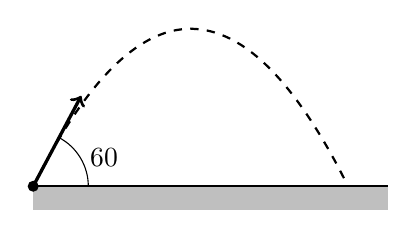
\begin{tikzpicture}
        \fill[gray!50] rectangle (4.5,-.3);
        \draw[thick](0,0)--(4.5,0);
        \fill circle(.07);
        \draw[thick,smooth,domain=0:4,dashed]
        plot({\x},{-.5*((\x-2)*(\x-2))+2});
        \draw[very thick,rotate=62,->](0,0)--(1.3,0);
        \draw(.7,0) arc(0:62:.7) node[midway,right]{\ang{60}};
      \end{tikzpicture}
    \end{center}
    \begin{choices}
      \choice\ang{30}
      \choice\ang{20} and \ang{80}
      \choice\ang{10} and \ang{120}
      \choice\ang{45} and \ang{135}
      \choice There is no other angle other than \ang{60} in which the ball will
      have a range of \SI{100}\metre.
    \end{choices}
    \vspace{.7in}
      
    \question A stack of coffee filters falls from rest through the air. Due to
    air resistance, the filters fall with an acceleration proportional to the
    velocity of fall, that is, $a=-kv$, where $k$ is a positive constant.
    The velocity of the falling filters as a function of time of fall is
    \begin{choices}
      \choice $-kv^2$
      \choice $-1⁄2kv^2$
      \choice $-k$
      \choice $\ln(kt)$
      \choice $v_0e^{-kt}$
    \end{choices}
    
%    \question A rubber ball is dropped from rest onto a plane angled at
%    $\theta=\ang{30}$ to the horizontal floor and bounces off the plane with a
%    horizontal speed $v_0$. The ball lands on the plane a distance $D$ along the
%    plane, as shown below. In terms of $v_0$, $D$, and $g$, the speed of the
%    ball just before striking the plane is
%    \cpic{.23}{bounce}
%    \begin{choices}
%      \choice $v_0$
%      \choice $\sqrt{v_0^2+2D\sin\theta g}$
%      \choice $\sqrt{v_0+\dfrac{D\sin\theta}g}$
%      \choice $\sqrt{v_0^2+\dfrac{D\sin\theta}g}$
%      \choice $\sqrt{2D\sin\theta g}$
%    \end{choices}
%  
%    \question A small ball is launched with a speed of \SI8{\metre\per\second}
%    at an angle of \ang{30} from the horizontal. A cup is hung so that it is in
%    position to catch the ball when it reaches its maximum height. How far
%    above the floor should the cup be hung to catch the ball?    
%    \cpic{.3}{cup}
%    \begin{choices}
%      \choice\SI{2.4}\metre
%      \choice\SI{1.6}\metre
%      \choice\SI{1.0}\metre
%      \choice\SI{.8}\metre
%      \choice\SI{.4}\metre
%    \end{choices}
%    
%    \question The velocity vs.\ time graph below represents the motion of a
%    bicycle rider. The displacement of the rider between $0$ and \SI4{\hour} is
%    \begin{center}
%      \begin{tikzpicture}[xscale=.8,yscale=.05]
%        \draw[thick,->](0,0)--(4.4,0) node[right]{$t$ (h)};
%        \draw[thick,->](0,-22)--(0,28)node[above]{$v$ (km/h)};
%        \foreach\x in {1,...,4} \draw(\x,2)--(\x,-2)node[below]{\x};
%        \foreach\y in {-20,-10,...,20} \draw(.1,\y)--(-.1,\y)node[left]{$\y$};
%        \draw[very thick](0,0)--(1,20)--(2,20)--(3,0)--(4,-20);
%        \draw[dotted](1,0)--(1,20);
%        \draw[dotted](2,0)--(2,20);
%      \draw[dotted](4,0)--(4,-20);
%      \end{tikzpicture}
%    \end{center}
%    \begin{choices}
%      \choice $+\SI{10}{\kilo\metre}$
%      \choice $+\SI{20}{\kilo\metre}$
%      \choice $+\SI{30}{\kilo\metre}$
%      \choice $+\SI{40}{\kilo\metre}$
%      \choice $-\SI{10}{\kilo\metre}$
%    \end{choices}

    \question An object starts from rest at $t=0$ and position $x=0$, then moves
    in a straight line with an acceleration described by the equation $a=4t^2$
    in \si{\metre\per\second\squared}. What is the position of the object at
    $t=\SI3\second$?
    \begin{choices}
      \choice\SI6\metre
      \choice\SI1\metre
      \choice\SI{27}\metre
      \choice\SI{54}\metre
      \choice\SI{108}\metre
    \end{choices}
    \columnbreak
    
    \uplevel{
      \textbf{Questions \ref{car1}--\ref{car2}}: A car of mass $m$ travels
      along a straight horizontal road. The car begins with a speed $v_0$, and
      accelerates according to the velocity function
      $v(t)=\sqrt{v_0^2+\dfrac{Ct^2}m}$, where $t$ is time, and $C$ is a
      positive constant.
    }

    \question The speed of the car is zero at a time $t$ of
    \begin{choices}
      \choice zero
      \choice $2t$
      \choice $4t$
      \choice $\sqrt{8t}$
      \choice The speed of the car is never zero.
    \end{choices}
    \label{car1}
    
    \question The acceleration of the car as a function of time is
    \begin{choices}
      \choice $v_0^2+\dfrac{Ct^2}m$
      \choice $v_0^2+\dfrac{2Ct^2}m$
      \choice $v_0+\dfrac{Ct}m$
      \choice $\dfrac{2Ct}m$
      \choice $\dfrac{2Ct^2}m$
    \end{choices}
    \label{car2}
  
    \question The motion of an object is represented by the acceleration vs.\
    time graph below. The object is intially at rest. Which of the following
    statements is true about the motion of the object?
    \begin{center}
      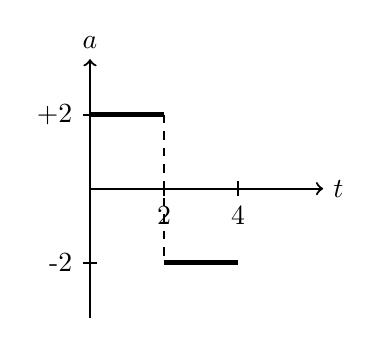
\begin{tikzpicture}[scale=.47,thick]
        \draw[->] (0,0)--(6.3,0) node[right]{$t$};
        \draw[->] (0,-3.5)--(0,3.5) node[above]{$a$};
        \draw[ultra thick](0,2)--(2,2);
        \draw[ultra thick](2,-2)--(4,-2);
        \draw[dashed] (2,2)--(2,-2);
        \draw (2,.2)--(2,-.2) node[below]{2};
        \draw (4,.2)--(4,-.2) node[below]{4};
        \draw (.2,2)--(-.2,2) node[left]{+2};
        \draw (.2,-2)--(-.2,-2) node[left]{-2};
      \end{tikzpicture}
    \end{center}
    \begin{choices}
      \choice The object returns to its original position.
      \choice The velocity of the object is zero at a time of \SI2\second.
      \choice The velocity of the object is zero at a time of \SI4\second.
      \choice The displacement of the object is zero at a time of \SI4\second.
      \choice The acceleration of the object is zero at a time of \SI2\second.
    \end{choices}
    \columnbreak

    \uplevel{
      \centering
      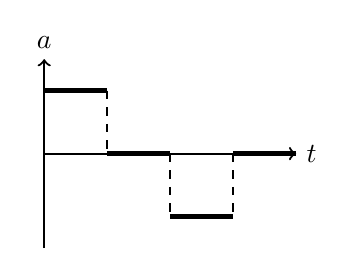
\begin{tikzpicture}[scale=.4,thick]
        \draw[->] (0,0)--(8,0) node[right]{$t$};
        \draw[->] (0,-3)--(0,3) node[above]{$a$};
        \draw[ultra thick](0,2)--(2,2);
        \draw[ultra thick](2,0)--(4,0);
        \draw[ultra thick](4,-2)--(6,-2);
        \draw[ultra thick](6,0)--(8,0);
        \draw[dashed] (2,2)--(2,0);
        \draw[dashed] (4,0)--(4,-2);
        \draw[dashed] (6,0)--(6,-2);
      \end{tikzpicture}
    }
    
    \question Which of the following pairs of graphs could show the position
    vs.\ time and velocity vs.\ time graphs for the acceleration vs. time graph
    shown above? Assume $v=0$ and $x=0$ at $t=0$.
    \begin{choices}
      \choice
      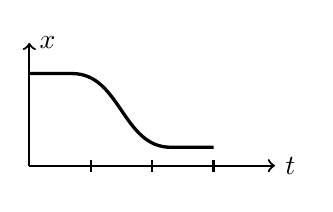
\begin{tikzpicture}[scale=.78,thick]
        \draw[->] (0,0)--(4,0) node[right]{$t$};
        \draw[->] (0,0)--(0,2) node[right]{$x$};
        \foreach \x in {1,2,3}\draw (\x,.1)--(\x,-.1);
        \draw[very thick](0,1.5)--(.7,1.5)to[out=0,in=180](2.3,.3)--(3,.3);
      \end{tikzpicture}
      \hspace{.2in}
      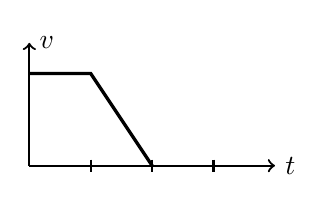
\begin{tikzpicture}[scale=.78,thick]
        \draw[->] (0,0)--(4,0) node[right]{$t$};
        \draw[->] (0,0)--(0,2) node[right]{$v$};
        \foreach \x in {1,2,3}\draw (\x,.1)--(\x,-.1);
        \draw[very thick] (0,1.5)--(1,1.5)--(2,0);
      \end{tikzpicture}

      \choice
      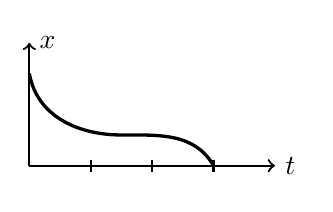
\begin{tikzpicture}[scale=.78,thick]
        \draw[->] (0,0)--(4,0) node[right]{$t$};
        \draw[->] (0,0)--(0,2) node[right]{$x$};
        \foreach \x in {1,2,3}\draw (\x,.1)--(\x,-.1);
        \draw[very thick](0,1.5)to[out=-80,in=180](1.5,.5)
        to[out=0,in=120](3,0);
      \end{tikzpicture}
      \hspace{.2in}
      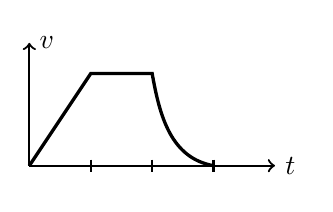
\begin{tikzpicture}[scale=.78,thick]
        \draw[->] (0,0)--(4,0) node[right]{$t$};
        \draw[->] (0,0)--(0,2) node[right]{$v$};
        \foreach \x in {1,2,3}\draw (\x,.1)--(\x,-.1);
        \draw[very thick](0,0)--(1,1.5)--(2,1.5) to[out=-80,in=170] (3,0);
      \end{tikzpicture}

      \choice
      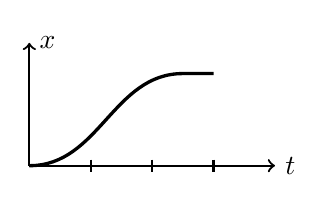
\begin{tikzpicture}[scale=.78,thick]
        \draw[->] (0,0)--(4,0) node[right]{$t$};
        \draw[->] (0,0)--(0,2) node[right]{$x$};
        \foreach \x in {1,2,3}\draw (\x,.1)--(\x,-.1);
        \draw[very thick] (0,0) to[out=0,in=180] (2.5,1.5)--(3,1.5);
      \end{tikzpicture}
      \hspace{.2in}
      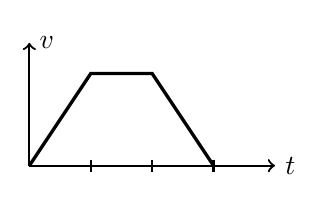
\begin{tikzpicture}[scale=.78,thick]
        \draw[->] (0,0)--(4,0) node[right]{$t$};
        \draw[->] (0,0)--(0,2) node[right]{$v$};
        \foreach \x in {1,2,3}\draw (\x,.1)--(\x,-.1);
        \draw[very thick] (0,0)--(1,1.5)--(2,1.5)--(3,0);
      \end{tikzpicture}

      \choice
      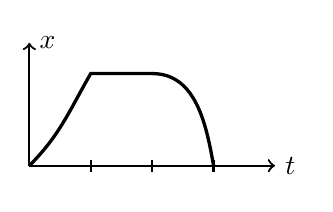
\begin{tikzpicture}[scale=.78,thick]
        \draw[->] (0,0)--(4,0) node[right]{$t$};
        \draw[->] (0,0)--(0,2) node[right]{$x$};
        \foreach \x in {1,2,3}\draw (\x,.1)--(\x,-.1);
        \draw[very thick](0,0) to[out=45,in=240] (1,1.5)--(2,1.5)
        to[out=0,in=100] (3,0);
      \end{tikzpicture}
      \hspace{.2in}
      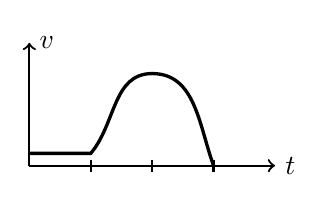
\begin{tikzpicture}[scale=.78,thick]
        \draw[->] (0,0)--(4,0) node[right]{$t$};
        \draw[->] (0,0)--(0,2) node[right]{$v$};
        \foreach \x in {1,2,3}\draw (\x,.1)--(\x,-.1);
        \draw[very thick] (0,.2)--(1,.2) to[out=50,in=180] (2,1.5)
        to[out=0,in=110] (3,0);
      \end{tikzpicture}

      \choice
      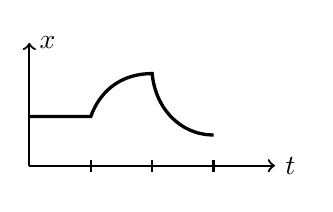
\begin{tikzpicture}[scale=.78,thick]
        \draw[->] (0,0)--(4,0) node[right]{$t$};
        \draw[->] (0,0)--(0,2) node[right]{$x$};
        \foreach \x in {1,2,3}\draw (\x,.1)--(\x,-.1);
        \draw[very thick] (0,.8)--(1,.8) to[out=70,in=180] (2,1.5)
        to[out=-85,in=180] (3,.5);
      \end{tikzpicture}
      \hspace{.2in}
      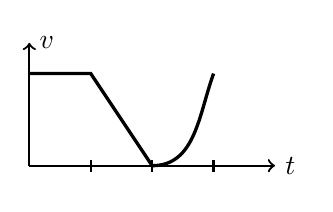
\begin{tikzpicture}[scale=.78,thick]
        \draw[->] (0,0)--(4,0) node[right]{$t$};
        \draw[->] (0,0)--(0,2) node[right]{$v$};
        \foreach \x in {1,2,3}\draw (\x,.1)--(\x,-.1);
        \draw[very thick](0,1.5)--(1,1.5)--(2,0) to[out=0,in=250] (3,1.5);
      \end{tikzpicture}
    \end{choices}
    \columnbreak
    
    \uplevel{
      \textbf{Questions \ref{q:fall1}--\ref{q:fall2}}: An object is released
      from rest and falls through a resistive medium. The resistance causes the
      velocity of the object to change according to the equation
      $v=16t-\dfrac12t^4$, where $v$ is in \si{\metre\per\second}, and time is
      in seconds.
    }

    \question Which of the following is a possible equation for the
    acceleration of the object as a function of time?
    \begin{choices}
      \choice $16-2t^2$
      \choice $16-2t^3$
      \choice $16-2t$
      \choice $8t^3-2t^2$
      \choice $32t^3-2t^5$
    \end{choices}
    \label{q:fall1}
    
    \question What is the terminal velocity of the object as it falls?
    \begin{choices}
      \choice \SI5{\metre\per\second}
      \choice \SI{10}{\metre\per\second}
      \choice \SI{24}{\metre\per\second}
      \choice \SI{32}{\metre\per\second}
      \choice The object never reaches a terminal velocity.
    \end{choices}
    \label{q:fall2}
    \columnbreak
  
    \question Two velocity vectors $v_1$ and $v_2$ each have a magnitude
    of \SI{10}{\metre\per\second}. Graph 1 shows the velocity $v_1$ at
    $t=\SI0\second$, and then the same object has a velocity $v_2$ at
    $t=\SI2\second$, shown in Graph 2. Which of the following vectors best
    represents the average acceleration vector that causes the object's velocity
    to change from $v_1$ to $v_2$ ?
    \begin{center}
      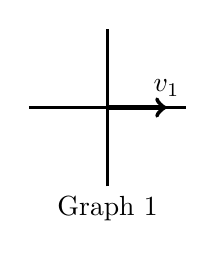
\begin{tikzpicture}[scale=.5,thick]
        \draw (-2,0)--(2,0);
        \draw (0,-2)--(0,2) node[pos=0,below]{Graph 1};
        \draw[ultra thick,->](0,0)--(1.5,0) node[above]{$v_1$};
      \end{tikzpicture}
      \hspace{.2in}
      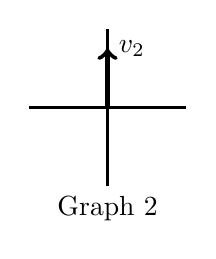
\begin{tikzpicture}[scale=.5,thick]
        \draw (-2,0)--(2,0);
        \draw (0,-2)--(0,2) node[pos=0,below]{Graph 2};
        \draw[ultra thick,->](0,0)--(0,1.5) node[right]{$v_2$};
      \end{tikzpicture}
    \end{center}
    
    \begin{choices}
      \choice
      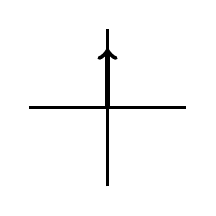
\begin{tikzpicture}[scale=.5,thick]
        \draw (-2,0)--(2,0);
        \draw (0,-2)--(0,2);
        \draw[ultra thick,->](0,0)--(0,1.5);
      \end{tikzpicture}
      \choice
      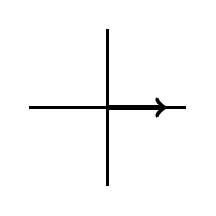
\begin{tikzpicture}[scale=.5,thick]
        \draw (-2,0)--(2,0);
        \draw (0,-2)--(0,2);
        \draw[ultra thick,->](0,0)--(1.5,0);
      \end{tikzpicture}
      \choice
      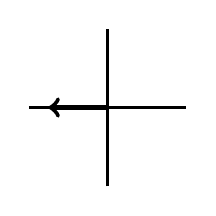
\begin{tikzpicture}[scale=.5,thick]
        \draw (-2,0)--(2,0);
        \draw (0,-2)--(0,2);
        \draw[ultra thick,->](0,0)--(-1.5,0);
      \end{tikzpicture}
      \choice
      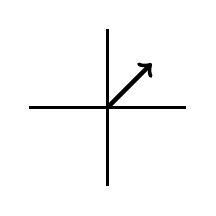
\begin{tikzpicture}[scale=.5,thick]
        \draw (-2,0)--(2,0);
        \draw (0,-2)--(0,2);
        \draw[ultra thick,->](0,0)--(1.12,1.12);
      \end{tikzpicture}
      \choice
      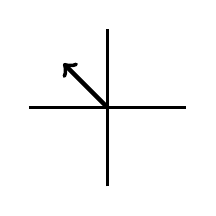
\begin{tikzpicture}[scale=.5,thick]
        \draw (-2,0)--(2,0);
        \draw (0,-2)--(0,2);
        \draw[ultra thick,->](0,0)--(-1.12,1.12);
      \end{tikzpicture}
    \end{choices}

    \question A toy dart gun fires a dart at an angle of \ang{45} to the
    horizontal and the dart reaches a maximum height of 1 meter. If the dart
    were fired straight up into the air along the vertical, the dart would
    reach a height of
    \begin{choices}
      \choice\SI1\metre
      \choice\SI2\metre
      \choice\SI3\metre
      \choice\SI4\metre
      \choice\SI5\metre
    \end{choices}
    \columnbreak
    
    \question The graph below shows the displacement as a function of time for a
    car moving in a straight line. Which of the following graphs shows the
    velocity vs.\ time graph for the same time intervals?
    \begin{center}
      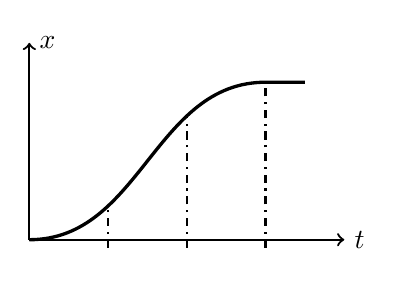
\begin{tikzpicture}[thick]
        \draw[->] (0,0)--(4,0) node[right]{$t$};
        \draw[->] (0,0)--(0,2.5) node[right]{$x$};
        \draw[very thick] (0,0) to[out=0,in=180] (3,2)--(3.5,2);
        \draw[dash dot] (3,-.1)--(3,2);
        \draw[dash dot] (2,-.1)--(2,1.6);
        \draw[dash dot] (1,-.1)--(1,.4);
      \end{tikzpicture}
    \end{center}
    \begin{choices}
      \choice
      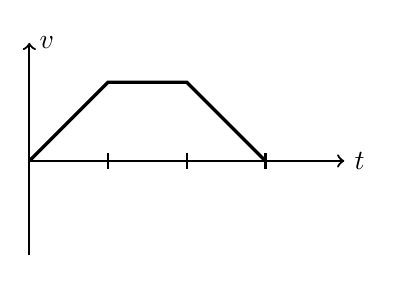
\begin{tikzpicture}[thick]
        \draw[->] (0,0)--(4,0) node[right]{$t$};
        \draw[->] (0,-1.2)--(0,1.5) node[right]{$v$};
        \foreach \x in {1,2,3}\draw (\x,.1)--(\x,-.1);
        \draw[very thick] (0,0)--(1,1)--(2,1)--(3,0);
      \end{tikzpicture}

      \choice
      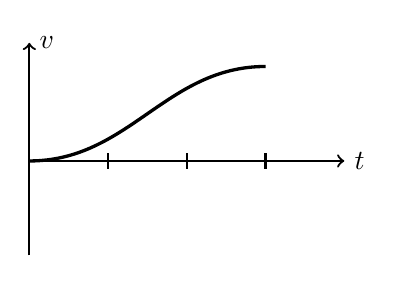
\begin{tikzpicture}[thick]
        \draw[->] (0,0)--(4,0) node[right]{$t$};
        \draw[->] (0,-1.2)--(0,1.5) node[right]{$v$};
        \foreach \x in {1,2,3}\draw (\x,.1)--(\x,-.1);
        \draw[very thick] (0,0) to[out=0,in=180] (3,1.2);
      \end{tikzpicture}

      \choice
      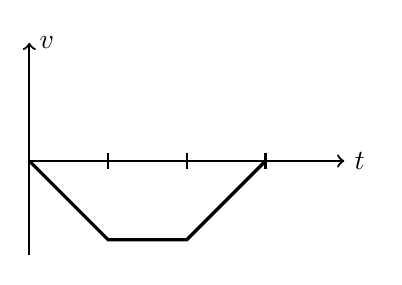
\begin{tikzpicture}[thick]
        \draw[->] (0,0)--(4,0) node[right]{$t$};
        \draw[->] (0,-1.2)--(0,1.5) node[right]{$v$};
        \foreach \x in {1,2,3}\draw (\x,.1)--(\x,-.1);
        \draw[very thick] (0,0)--(1,-1)--(2,-1)--(3,0);
      \end{tikzpicture}

      \choice
      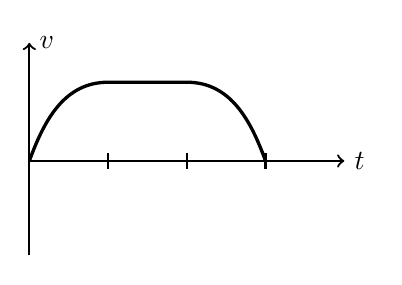
\begin{tikzpicture}[thick]
        \draw[->] (0,0)--(4,0) node[right]{$t$};
        \draw[->] (0,-1.2)--(0,1.5) node[right]{$v$};
        \foreach \x in {1,2,3}\draw (\x,.1)--(\x,-.1);
        \draw[very thick] (0,0) to[out=70,in=180] (1,1)--(2,1)
        to[out=0,in=110] (3,0);
      \end{tikzpicture}
      
      \choice
      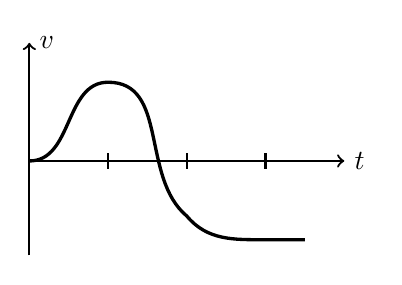
\begin{tikzpicture}[thick]
        \draw[->] (0,0)--(4,0) node[right]{$t$};
        \draw[->] (0,-1.2)--(0,1.5) node[right]{$v$};
        \foreach \x in {1,2,3}\draw (\x,.1)--(\x,-.1);
        \draw[very thick] (0,0) to[out=0,in=180] (1,1) to[out=0,in=140] (2,-.7)
        to[out=-50,in=180] (3,-1)--(3.5,-1);
      \end{tikzpicture}
    \end{choices}
  \end{questions}
  \setcounter{lastmc}{\value{question}}    
\end{multicols*}
\newpage

%\genfreetitle{1}{KINEMATICS}{3}
%\genfreedirections

\begin{questions}
  \setcounter{question}{\value{lastmc}}
  
  \question The position $x$ of an object is described with respect to time $t$
  by the following equation: $x=2t^3-15t^2+36t-8$, where $x$ is in meters and
  $t$ in seconds. Answer the following questions.
  \begin{parts}
    \part Find its displacement between $t=3$ and \SI5\second.
    \vspace{\stretch1}
    
    \part Write out an expression for the velocity of the object with respect to
    time.
    \vspace{\stretch1}
    
    \part Write out an expression for the acceleration of the object with
    respect to time.
    \vspace{\stretch1}
    
    \part At what point(s) in time is the velocity of the object zero?
    \label{partd}
    \vspace{\stretch1}
    
    \part At each of those points (from \ref{partd} above), is the acceleration
    positive, negative, or zero?
    \vspace{\stretch1}
    \part During what intervals of time is the velocity of the object positive?
    \vspace{\stretch1}
    
    \part During what intervals of time is the acceleration of the object
    positive?
    \vspace{\stretch1}
    \newpage
  \item On the graph (on the next page), sketch position $x$, velocity $v$ and
    acceleration $a$ as functions of time.
  \end{parts}
  \begin{center}
    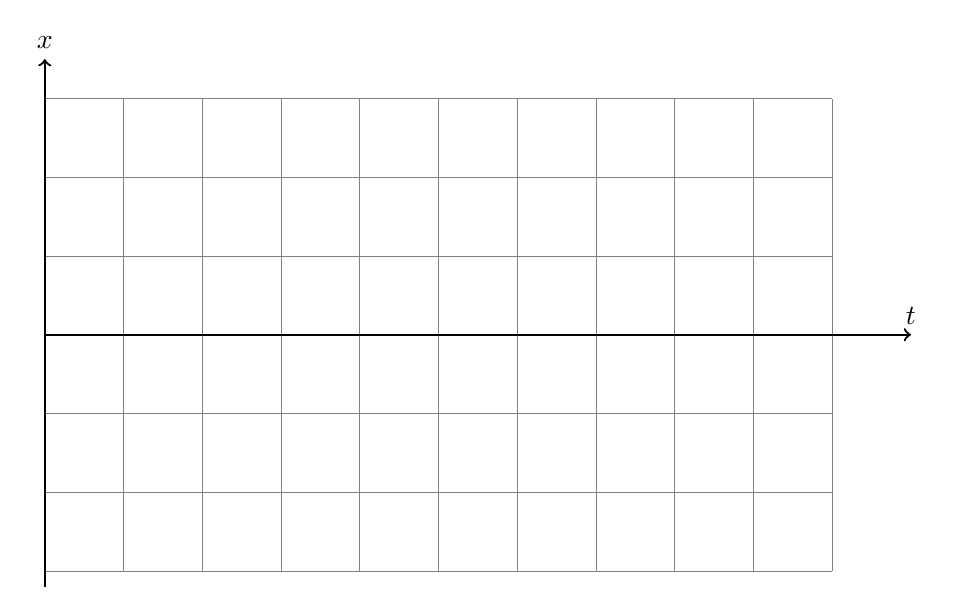
\begin{tikzpicture}
      \draw[help lines](0,-3) grid(10,3);
      \draw[thick,->](0,-3.2)--(0,3.5) node[above]{$x$};
      \draw[thick,->](0,0)--(11,0) node[above]{$t$};
    \end{tikzpicture}

    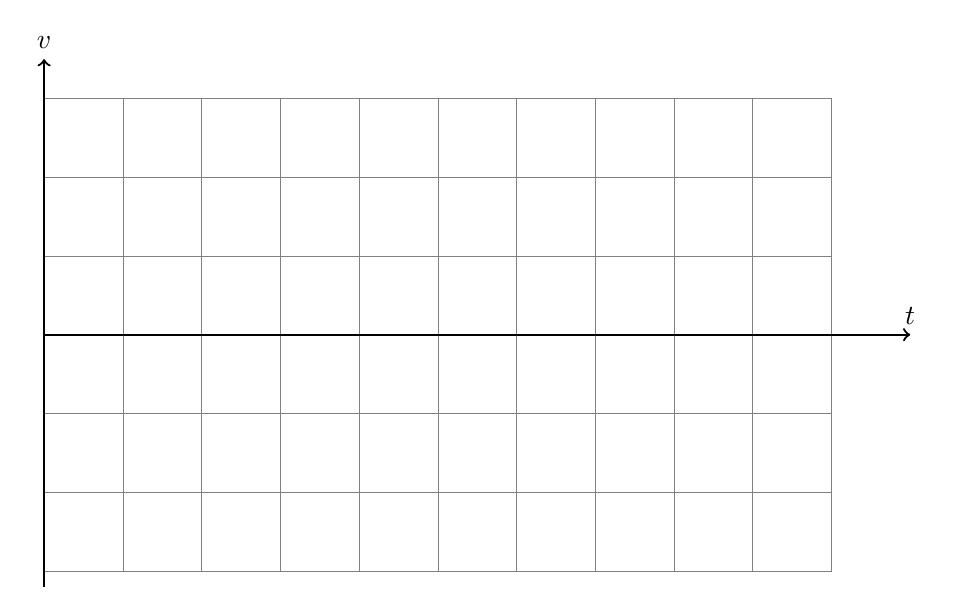
\begin{tikzpicture}
      \draw[help lines](0,-3) grid(10,3);
      \draw[thick,->](0,-3.2)--(0,3.5) node[above]{$v$};
      \draw[thick,->](0,0)--(11,0) node[above]{$t$};
    \end{tikzpicture}

    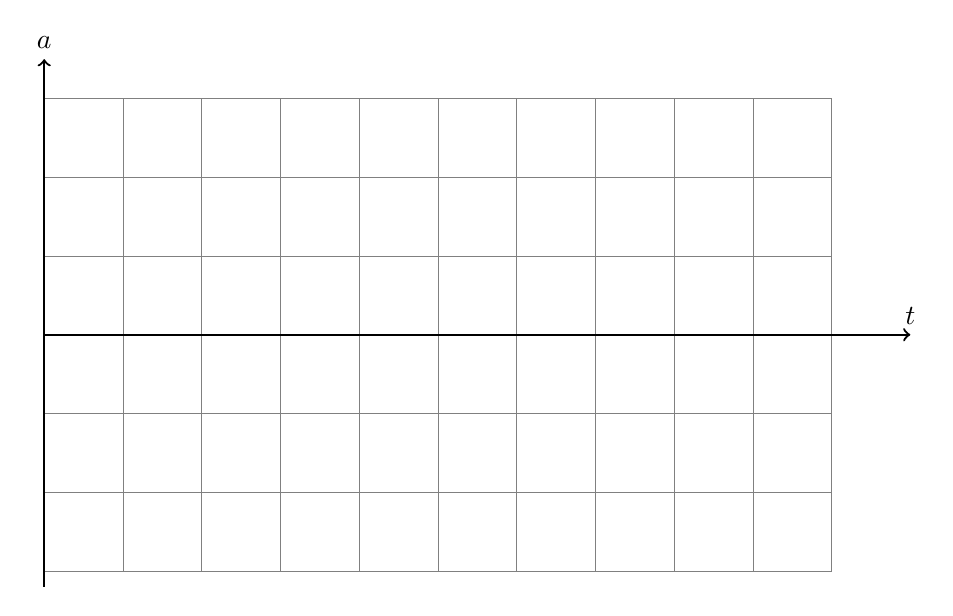
\begin{tikzpicture}
      \draw[help lines](0,-3) grid(10,3);
      \draw[thick,->](0,-3.2)--(0,3.5) node[above]{$a$};
      \draw[thick,->](0,0)--(11,0) node[above]{$t$};
    \end{tikzpicture}
  \end{center}
  \newpage

%  \question A steel ball is dropped from a point with $(x,y)$ coordinate of
%  $(\SI8\metre,\SI{16}\metre)$. At the same time, another ball is launched
%  from the origin with a speed of \SI{20}{\metre\per\second} at an angle of
%  \ang{30}.
%  \begin{parts}
%    \part Find the minimum distance of separation occur of the two balls.
%    \part At what time does this separation occur?
%    \part Give the coordinates of the two balls for the minimum separation.
%  \end{parts}
%  \newpage

  % TAKEN FROM 2015 AP PHYSICS C FREE-RESPONSE QUESTION MECH 1
  \cpic{.5}{motion-sensor}

  \question A block of mass $m$ is projected up from the bottom of an inclined
  ramp with an initial velocity of magnitude $v_0$. The ramp has negligible
  friction and makes an angle $\theta$ with the horizontal. A motion sensor
  aimed down the ramp is mounted at the top of the incline so that the positive
  direction is down the ramp. The block starts a distance $D$ from the motion
  sensor, as shown above. The block slides partway up the ramp, stops before
  reaching the sensor, and then slides back down.
  \begin{parts}
    \part Consider the motion of the block at some time $t$ after it has been
    projected up the ramp. Express your answers in terms of $m$, $D$, $v_0$,
    $t$, $\theta$ and physical constants, as appropriate.
    \begin{subparts}
      \subpart Determine the acceleration $a$ of the block.
      \vspace{\stretch1}
      
      \subpart Determine an expression for the velocity $v$ of the block.
      \vspace{\stretch1}
      
      \subpart Determine an expression for the position $x$ of the block.
      \vspace{\stretch1}
    \end{subparts}

    \part Derive an expression for the position $x_\text{min}$ of the block when
    it is closest to the motion sensor. Express your answer in terms of $m$,
    $D$, $v_0$, $\theta$, and physical constants, as appropriate.
    \vspace{\stretch2}
    \newpage
    
    \part On the axes provided below, sketch graphs of position $x$, velocity
    $v$, and acceleration $a$ as functions of time $t$ for the motion of the
    block while it goes up and back down the ramp. Explicitly label any
    intercepts, asymptotes, maxima, or minima with numerical values or
    algebraic expressions, as appropriate.
    \begin{center}
      \begin{tikzpicture}[scale=1.8,very thick,->]
        \draw (0,0)--(2.5,0)  node[right]{$t$};
        \draw (0,-1.5)--(0,1.5) node[above]{$x$};
      \end{tikzpicture}
      \hspace{.2in}
      \begin{tikzpicture}[scale=1.8,very thick,->]
        \draw (0,0)--(2.5,0)  node[right]{$t$};
        \draw (0,-1.5)--(0,1.5) node[above]{$v$};
      \end{tikzpicture}
      \hspace{.2in}
      \begin{tikzpicture}[scale=1.8,very thick,->]
        \draw (0,0)--(2.5,0)  node[right]{$t$};
        \draw (0,-1.5)--(0,1.5) node[above]{$a$};
      \end{tikzpicture}
    \end{center}
    
    \part After the block slides back down and leaves the bottom of the ramp, it
    slides on a horizontal surface with a coefficient of friction given by
    $\mu_k$. Derive an expression for the distance the block slides before
    stopping. Express your answer in terms of $m$, $D$, $v_0$, $\theta$,
    $\mu_k$, and physical constants, as appropriate.
    \vspace{\stretch1}
    
    \part Suppose the ramp now has friction. The same block is projected up with
    the same initial speed $v_0$ and comes back down the ramp. On the axes
    provided below, sketch a graph of the velocity $v$ as a function of time $t$
    for the motion of the block while it goes up and back down the ramp,
    arriving at the bottom of the ramp at time $t_f$. Explicitly label any
    intercepts, asymptotes, maxima, or minima with numerical values or
    algebraic expressions, as appropriate.
    \begin{center}
      \begin{tikzpicture}[scale=1.8,very thick,->]
        \draw (0,0)--(2.5,0)  node[right]{$t$};
        \draw (0,-1.5)--(0,1.5) node[above]{$v$};
      \end{tikzpicture}
    \end{center}
    \vspace{\stretch{.5}}
  \end{parts}
  \newpage
  
  % TAKEN FROM 2010 AP PHYSICS C FREE-RESPONSE QUESTION MECH 3
  \uplevel{
    \cpic{.3}{skier}
  }

  \question A skier of mass $m$ will be pulled up a hill by a rope, as shown
  above. The magnitude of the acceleration of the skier as a function of time
  $t$ can be modeled by the equations
  \begin{align*}
    a &=a_\text{max}\sin\left(\frac{\pi t}T\right)  &(0<t<T)&\\
    &=0 & (t\geq T)&
  \end{align*}
  where $a_\text{max}$ and $T$ are constants. The hill is inclined at an angle
  $\theta$ above the horizontal, and friction between the skis and the snow is
  negligible. Express your answers in terms of given quantities and fundamental
  constants.
  \begin{parts}
    \part  Derive an expression for the velocity of the skier as a function of
    time during the acceleration. Assume the skier starts from rest.
    \vspace{\stretch1}
    
    \part Derive an expression for the work done by the net force on the skier
    from rest until terminal speed is reached.
    \vspace{\stretch1}
    
    \part Determine the magnitude of the force exerted by the rope on the skier
    at terminal speed.
    \vspace{\stretch1}
    
    \part Derive an expression for the total impulse imparted to the skier
    during the acceleration.
    \vspace{\stretch1}
    \newpage
    
    \part Suppose that the magnitude of the acceleration is instead modeled as
    $a=a_\text{max}e^{-\pi t/2T}$ for all $t>0$, where $a_\text{max}$ and $T$
    are the same as in the original model. On the axes below, sketch the graphs
    of the force exerted by the rope on the skier for the two models, from
    $t=0$ to a time $t>T$. Label the original model $F_1$ and the new model
    $F_2$.
    \begin{center}
      \begin{tikzpicture}[thick]
        \draw[->] (0,0)--(10,0)node[right]{$t$};
        \draw[->] (0,0)--(0,6) node[above]{$F$};
        \draw (-.2,1.5)--(.2,1.5)node[pos=0,left]{$mg\sin\theta$};
        \draw (5.5,-.2)--(5.5,.2)node[pos=0,below]{$T$};
      \end{tikzpicture}
    \end{center}
    \vspace{\stretch1}
  \end{parts}
\end{questions}
\end{document}
